\section{Parity, and Parity Violation}
\subsection{Parity} 
 Parity, denoted by \ps, is the operation of replacing all space
 coordinates $x, y, z$ with $-x, -y, -z$, which is the effect of a mirror
 reflection followed by a \degrees{180} rotation.

 What we mean with parity symmetry is that the laws of physics should
 be symmetric. This means in practise that if you build an experiment
 with result x, then the mirror-reflected experiment should yield the
 mirror-reflected result.

 An example of a physical law that is symmetric under parity is
 gravity:
\begin{equation}
 m \frac{d^2 \vec{x}}{dt^2} = -G \frac{\vec{x}-\vec{y}}{|\vec{x}-\vec{y}|} 
 \frac{Mm}{|\vec{x}-\vec{y}|^2}
\end{equation}
 where $\vec{x}$ represents the position of some object with mass $m$
 (say earth) and $\vec{y}$ the position of another object with mass
 $M$ (e.g. the sun). Replace all co-ordinates with their negatives,
 i.e. \(\vec{x} \topar -\vec{x}\) and \(\vec{y} \topar -\vec{y}\) and
 the equation remains valid and the same. This is what's meant with
 parity symmetry. What matters is that the laws are invariant.  The
 fact that the two objects $m$ and $M$ find themselves in a different
 position after the parity operation does not violate parity. However,
 if they were now governed by different laws of physics, e.g. if they
 were suddenly not subject to the gravitational force anymore, that
 would violate parity. A thought experiment that would test for parity
 is to take two system, one the exact mirror image of the other. If
 the two evolve such that they remain exact mirror images of each
 other, parity is not violated. If they differ after a while, it is
 violated. 
 %Of course there are practical reasons why it is impossible to set up experiments that are such exact mirror images that they'd remain mirror images for all times, even if parity is not violated. This is the sort of thing an experimenter will have to take into account when evaluation the outcome of a real experiment, not a thought experiment, though.

 Parity is a discrete symmetry, as opposed to a continuous
 symmetry. Continuous symmetry operations can be build up by a
 succession of infinitesimally small steps. Examples are, for example,
 rotations, and the associated conserved quantity is angular
 momentum. The conservation of such symmetries is very fundamental to
 our understanding of physics. Mirror reflection however is a discrete
 symmetry operation - there is no continuous path to transform an
 object into its own mirror image, you'll have to break it apart and
 build it from scratch. So, while a rotated object (or experiment) can be considered
 to be the same object as before the rotation, a mirror reflected
 object (or experiment) cannot, it is a different thing. This makes discrete
 symmetries fundamentally different from continuous ones, and there is
 clearly less reason to assume that they are good symmetries of
 nature.

 However, all physical interactions governing our every-day life are
 in fact mirror symmetric (gravity and electromagnetism) so the idea
 that parity is a fundamental symmetry of nature seems - well,
 natural. But, as we will see below, it is wrong. 

\subsection{The effect of parity on various quantities}

\paragraph{Position} That's how we defined it: 
\[ \vec{x} \topar -\vec{x} \]
\paragraph{velocity} Same thing, since $\vec{v} = \dbyd{}{t} \vec{x}$, so
\[ \vec{v} \topar -\vec{v} \]
\paragraph{mass} Remains the same - we \emph{define} the rest-mass as
 a property of the body, independent of its position.
\paragraph{momentum} of course the same as velocity
\[ \vec{p} \topar -\vec{p} \]
\paragraph{Energy} Remains the same. Intuitively clear, but also
 mathematically: Non-relativistically \( E = m\vec{v}^2 \), clearly
 invariant.  Similarly, relativistically, \(E = \sqrt{ m^2 +
 \vec{p}^2}\), also remains the same.
\[ E \topar E \]
\paragraph{angular momentum} More interesting:
\[ \vec{L} = \vec{r} \times \vec{p} \topar (-\vec{r})
\times (-\vec{p}) = \vec{r} \times \vec{p} = \vec{L},
\] so angular momentum is invariant under parity:
\[\vec{L} \topar \vec{L}\]
This is the defining property of an \textbf{axial vector}, or pseudo vector (while $\vec{x}$, $\vec{p}$ are simply vectors).
\paragraph{Electric field $\vec{E}$}
The electric field at $\vec{r}$ due to a point charge $q$ at the origin is:
\[
    \vec{E} = \frac{q}{4\pi\epsilon_0} \frac{\vec{r}}{|\vec{r}|}\frac{1}{|\vec{r}|^2}
\]
So 
\[
    \vec{E} \topar -\vec{E}  
\]
This can be more generically derived from Maxwell's equations, but for the purpose of these notes, we'll be satisfied with noting that
this remains true for a charge moving with speed $v$:
\[
    \vec{E} = \frac{q}{4\pi \epsilon_0} \frac{1-v^2/c^2}{(1-v^2\sin^2\theta/c^2)^{3/2}}
    \frac{\vec{r}}{|\vec{r}|}
    \frac{1}{|\vec{r}|^2}.
\]
\paragraph{Magnetic field $\vec{B}$}
The magnetic field due to a charge moving with velocity $\vec{v}$ is given by
\[
    \vec{B} = \frac{1}{c^2} \vec{v} \times \vec{E} 
\]
Since $\vec{v} \topar -\vec{v}$ and $\vec{E} \topar -\vec{E}$, we have
\[
    \vec{B} \topar \vec{B}
\]
So the magnetic field vector is an axial vector.
%%


\subsection{Parity in particle physics}
\label{sec:ParityInPP}
\subsubsection{Parity of individual particles}
Particles are described by a quantum mechanical wave function. How does this transform? This derives directly from the transformation properties of the parameters the wave function depends on, so in the position representation, we get:
\begin{equation}
    \psi(x, y, z) \topar \psi'(x, y, z) = \psi(-x, -y, -z)
\end{equation}
Because fundamental particles are point-like objects which have no structure of shape, they should be mirror-symmetric. Therefore, a fundamental particle at rest must transform into itself under parity.  For the wave function it means that
\begin{equation}
 \left|\psi \right|^2 \topar \left|\psi\right|^2
\end{equation}
Note that this is a relationship between the absolute squared of the wave-functions, which is the observable quantity. For the wave function this implies
\begin{equation}
 \psi \topar e^{i\phi} \psi
\end{equation}
 or equivalently
\begin{equation}
 \ps \psi = e^{i\phi} \psi
\end{equation}
This means that a wavefunction $\psi$ describing a single fundamental particle must be an eigenfunction of the parity operator \ps. Since $\ps^2=1$ (two mirror reflections = identity), $\ps^2$ has only one eigenvalue, which is $1$. Therefore \ps\ must have eigenvalues whose square is $1$. So the eigenvalues of \ps\ are $1$ and $-1$.
\begin{figure}
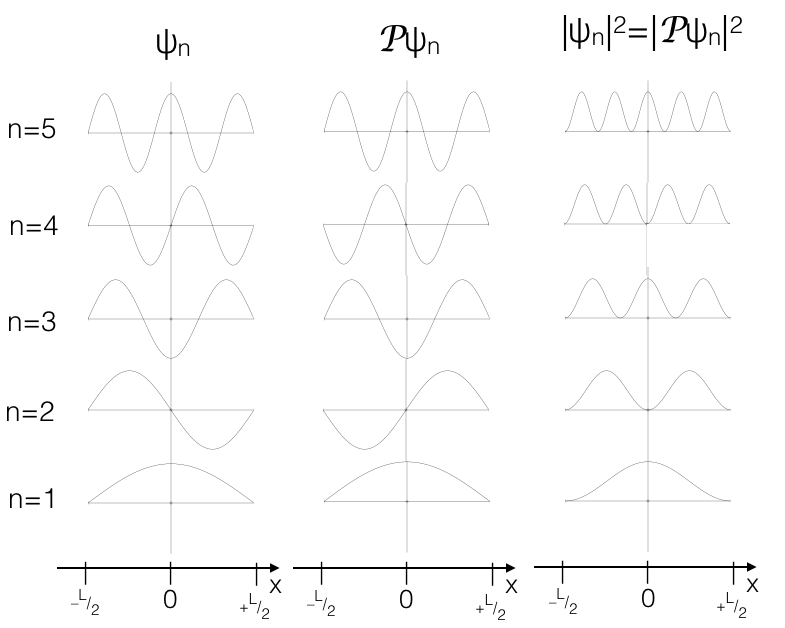
\includegraphics[width=0.9\textwidth]{fig/Parity_1D_squareWell}
\caption{The effect of parity on the wave functions describing a particle in an infinite square well of length $L$, in one dimension. The solutions to the Schr\"odinger equation are: $\psi_n(x)=\sin(n \pi (x/L + \half))$. The wave function $\psi_n$ is parity-odd (i.e $\ps \psi_n(x) = -\psi_n(x)$) for $n = 1, 3, 5 , \ldots$ and parity-even (i.e $\ps \psi_n(-x) = +\psi_n(x)$) for $n = 2, 4, 6, \ldots$. Note that in the analogy we use here, each $\psi_n$ corresponds to a different particle.
\label{fig:parity_1D_squareWell}}
\end{figure}
Let us have a look at a wave function of a particle in a 1-dimensional infinite square well, shown in \figref{fig:parity_1D_squareWell}. Because the square well is symmetric with respect to reflections about $x=0$, we require $|\psi_n(-x)|^2=|\psi_n(x)|^2$, which we do indeed find in the solution: $\psi_n(x)=\sin(n \pi (x/L + \half))$. The wave function $\psi_n$ is parity-odd (i.e $\ps \psi_n(x) = -\psi_n(x)$) for $n = 1, 3, 5 , \ldots$ and parity-even (i.e $\ps \psi_n(-x) = +\psi_n(x)$) for $n = 2, 4, 6, \ldots$. Note that in the analogy we use here, each $\psi_n$ corresponds to a different particle (rather than one and the same particle in a different energy states). In reality, particles move in 3 spatial dimension, and we demand symmetry about their own origin, i.e. $|\psi(x,y,z)|^2 = |\psi(-x,-y,-z)|^2$, leaving us with...\\
\fbox{\parbox{0.98\textwidth}{
 Two kinds of particle
 wavefunctions, one picks up a '$-$' sign under parity (parity odd), the other does not (parity even).
 }}
\begin{equation}
\begin{array}{rcrl}
 \psi& \topar & \psi & \mbox{even intrinsic parity}
\\
 \psi& \topar & -\psi & \mbox{odd intrinsic parity}
\end{array}
\end{equation}
 Both exist in nature. In the formula sheet at the back you find a list of particles, and for each the $J^{PC}$ quantum numbers are given. 
 $J$ is the spin of the particles. $P$ is its parity eigenvalue. The meaning of $C$ (which is not defined for all particles, in which case only $J^P$ is given), will be discussed very soon. 
 Looking at the quantities we know, we find that the $\pi^+$, for example, has $J^{P} = 0^-$, which means it is a spin zero particle which is parity-odd, i.e. has parity eigenvalue $-1$. The $f_0(980)$ has $J^{PC}=0^{++}$, so it is also spin zero, but parity-even (and it also as $C=+1$, but as mentioned previously, we learn about the meaning of that later). 
 You will not find a parity value for electrons, muons, etc. There you use instead the following rule:
 \fbox{\parbox{0.9\textwidth}{
 Fermions have
 always the opposite parity of their antiparticles, so fermion
 anti-fermion pairs (like $e^+ e^-$) always have combined negative intrinsic parity. (The full parity value of the system also depends on the angular momentum as described below.)
}}

 \subsubsection{Parity of a two-particle system}
 You are familiar with a very famous two-particle system from your quantum mechanics course, the Hydrogen atom. This can be solved by reducing it to a one-particle problem of an electron (with reduced mass) in a $1/r^2$ potential. The solutions in spherical coordinates are of the form
 \begin{equation}
  \psi(r, \theta, \phi) = f(r) Y^{m}_{L}(\theta, \phi)
 \end{equation}
 \begin{figure}
 \begin{tabular}{ccc}
 \parbox{0.4\textwidth}{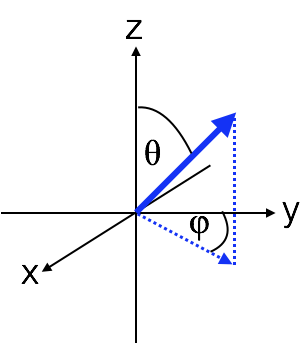
\includegraphics[width=0.4\textwidth]{fig/Parity_sphericalCoord_before}}
& {\Huge \topar} &
 \parbox{0.4\textwidth}{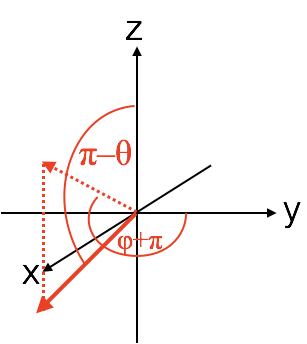
\includegraphics[width=0.4\textwidth]{fig/Parity_sphericalCoord_after}}
 \end{tabular}
 \caption{Spherical Coordinates under Parity.\label{fig:sphericals_under_parity}}
 \end{figure}
 So it factorises in a part that depends on the radial distance $r$ described by $f(r)$, and in another that depends on the angles $\theta$ and $\phi$. That latter part is $Y^{m}_{L}(\theta, \phi)$, the spherical harmonic function labelled by the orbital angular momentum quantum number $L$ and the magnetic quantum number $m$. Spherical coordinates transform under parity like this (see \figref{fig:sphericals_under_parity}):
 \begin{eqnarray}
    r & \topar & r \nonumber\\
    \theta & \topar & \pi - \theta \nonumber \\
    \phi & \topar & \phi + \pi
 \end{eqnarray}
 So, under parity, nothing is going to happen to $f(r)$. For the spherical harmonic, it turns out
 \begin{equation}
  Y^{m}_{L}(\theta, \phi) \topar 
  Y^{m}_{L}(\pi-\theta, \phi+\pi)
  = (-1)^L Y^{m}_{L}(\theta, \phi)
 \end{equation}
 So $Y^{m}_{L}$, and hence the entire wavefunction describing the electron-nucleus system, is parity even for $L=0, 2, 4, \ldots$ and it is parity odd for $L=1, 3, 5, \ldots$. 
 
 
 The factorisation of the solution into an $r$-dependent part and a spherical harmonic, $\psi(r, \theta, \phi) = f(r) Y^{m}_{L}(\theta, \phi)$, is not specific to the hydrogen atom, it results directly from the symmetry of the problem and generalises to any two-particle systems composed of point particles (which is the approximation being made when you derive this for the Hydrogen atom).
 So we can generalise our observation to the sweeping statement: The parity of a two-particle system is $(-1)^L$ \emph{multiplied} with the intrinsic parity eigenvalues of the constituents. This result is so important, we repeat it in a box:\\
 \fbox{\parbox{0.98\textwidth}{
\paragraph{Key result: The parity (P) eigenvalue of a two body system}
If each particle is a P eigenstate.
\[
P = (-1)^{L} \times \prod\limits_{\mathsf{all\;particles}} \mbox{(intrinsic parity)}
\]
The intrinsic parity of a fermion-antifermion pair is $-1$, so, for a pair of spin-\half\ fermions $P =(-1)^{L+1}$. For a pair of pions, which each have intrinsics parity $-1$, the overall parity value is $P=(-1)^L$.
}}
So, for example two pions in an $L=0$ state have parity $+1$. Two pions in an $L=1$ state have parity eigenvalue $-1$. A pion and an $f_0(980)$ in a $L=0$ state have parity $-1$, etc.

\paragraph{Parity of three and more-body systems}
To calculate the parity of systems with more than two particles, we break down the problem into successive 2-body problem. So we group particles into pairs, calculating the parity of each pair, $P_i$, and then treat each pair as if it were a single particle with intrinsic parity $P_i$, and repeat until we have only two particles left. This is best explained by example. Consider $\pi^+ \pi^- \pi^0$.

Let us treat this as \prt{\pi^+ \pi^-} pair plus a $\pi^0$. The \prt{\pi^+ \pi^-} pair has intrinsic $P_{1\,\mathsf{intrinsic}}=(-1)\cdot(-1)=+1$. Let us assume that the $\pi^+ \pi^-$ system has angular momentum quantum number $L_1$. Then its total parity of the $\pi^+ \pi^-$ system is $P_1 = (-1)^{L_1} \cdot (+1)=(-1)^{L_1}$.

The intrinsic parity of the \prt{\pi^0} is $-1$. Let's call the angular momentum of the $\pi^0$ relative to the \prt{\pi^+ \pi^-} pair $L_2$. Then the total parity of the three particle system is $P = P_1 \cdot (-1) \cdot (-1)^{L_2}= (-1)^{L_1 + L_2 + 1}$
To evaluate $P$ from this, we need to know something about $L_1, L_2$. Usually we do now know $L_1$, $L_2$ individually, but we do know the total angular momentum of the system.

Let us first consider the case where the three pions result from the decay of a spin zero particle, as in \prt{D^0 \to \pip\pim\piz}. Then the total $L+S$ of the three pion system must be $0$. Because the pions all have spin $0$, $L=0$. For a given pair of values $L_1, L_2$, the total angular momentum of the system, $L$, can have values 
$L = |L_1 - L_2|, \ldots, L_1 + L_2$. So $L=0$ is only possible if $L_1 = L_2$. Hence $P =  (-1)^{2L_1 + 1} = -1$

The situation is more complicated with a three pion system with overall $L=1$ (which is what we could get if it results from the decay of a spin-1 particle), which can have different parities, depending on the relative angular momenta between the particles that make up the overall $L=1$ state. For example, the \prt{\pi^+\pi^-} system could be in an $L_1 =1$ state. Then the relative angular momentum between the \prt{(\pi^+\pi^-)} system and the \piz\ can be $L_2 = 0, 1, 2$ without violating angular momentum conservation. The parity of the system is even for the $L_2 = 0$ and $L_2 = 2$ case, and odd for the $L_2 = 1$ case.

(In contrast to last year, you will not be asked to calculate the parity of three or more body systems in the exam with an initial state with $J=1$, but you should still know the basic ideas and results.)

\subsection{Parity Symmetry and Conservation}
 As you will remember from Quantum Mechanics, every symmetry comes
 with a conservation law. If parity were a good symmetry, it would
 imply that the commutator between the Hamiltonian that describes our
 parity-symmetric physics, and the parity operator, vanishes.
\begin{equation}
 \left[\ps, H\right] = 0
\end{equation}
 This has two consequences for a conserved symmetry:
\begin{itemize}
 \item If \ps\ is a good symmetry it can be measured simultaneously
   with energy/mass, so \ps\ is a good quantum number and for any
   particle one should be able to measure both its parity and its mass.
 \item If \ps\ is a good symmetry parity would be conserved, i.e. if a state is
 parity even, it will always remain parity even (even after a particle decay, for example), and if a state is parity odd, it will always parity
 odd. A parity odd unstable particle would always decay to a parity
 odd final state, a parity even one always into a parity even final
 state.
\end{itemize}

If parity is a good symmetry of nature, parity must be conserved in particle decays. To decide if a particle decay conserves parity we need to evaluate the parity before and after the decay. For this, we need to consider the parity eigenvalues given in the formula sheet, and we need to figure out the possible angular momentum states of any multi-particle system.

\paragraph{Example}
Let us consider $f_0(980) \to \pi^+ \pi^-$. The parity of the initial state is given to us in the formula sheet. For the $f_0(980)$ we find $J^P = 0^+$ (where $J=$spin and $P = \pm$ for parity even/odd), so it is parity-even. The $J^P$ of the pions is $0^-$. 
To evaluate the parity of the final state we need to know the angular momentum. Because $\vec{L}+\vec{S}$ is conserved, and all particles involved have spin ($J=0$), $L$ must be zero. So the parity of the final state is
\[
P = (-1)^{0} \times (-1) \times (-1) = +1
\]
which is the same as the initial state. Hence Parity is conserved in this decay.

\paragraph{Example}
Let us consider $K^+ \to \pi^+ \pi^0$. For the \prt{K^+}, $J^P = 0^-$, so the parity of the initial state is $-1$. The $J^P$ of the pions is $0^-$.  The $\eta$ has spin $J=0$, as do the pions, therefore, due to angular momentum conservation, $L$ must be zero. So the parity of the final state is
\[
P = (-1)^{0} \times (-1) \times (-1) = +1
\]
which is not the same as the initial state. Hence Parity is violated in this decay.

\paragraph{Example}
Consider $\rho \to \pi^+ \pi^-$. The $\rho$ had $J^P=1^-$. So it is parity odd. The pions have $J^P=0^-$, so they are each parity odd. Because the $\rho$ has $J=1$ and the pions have each $J=0$, the angular momentum quantum number of the two-pion system must be $L=1$. Hence the final state parity is:
\[
P = (-1)^{1} \times (-1) \times (-1) = -1
\]
which is the same as the initial state. Hence Parity is conserved in this decay.

\paragraph{Example}
Consider $D^0 \to \rho^+(770) \rho^-(770)$. The \prt{D^0} has $J^{P}=0^-$. So it is parity-odd. The $\rho$ mesons have $J^P=1^-$. Because each $\rho$ has $J=1$, they can combine to a total spin of $S=0$, $1$, or $2$. Because the inital state was $J=0$, the angular momentum needs to compensate for the spin, leading to $\vec{L}+\vec{S}=0$. This means $L$ can be either $0,1,2$.
\[
P = (-1)^{L} \times (-1) \times (-1) = (-1)^L
\]
Depending on $L$, the final state is therefore either parity odd ($L=1$) or even ($L=0,2$). This means that (if we don't know $L$), the observation of this decay would be compatible with parity conservation, as the final state can have the same parity as the initial state.

Parity conservation was the assumed to be true
 for a long time. Then came the $\tau-\theta$ puzzle, and eventually Wu's experiment. But let's first practice our parity violation detection skills:\\
\exercise{\textbf{Parity violating decay or not?}
For the following decays, decide whether the decay violates parity or not. You can find the spin and parity eigenvalues of the particles involved in the formula sheet in the format and $J^P$ where $J$ is the spin, and $P$ indicates whether it's a positive ($+$) or negative ($-$) parity eigenstate. For particles that are their own antiparticle you find two signs in the exponent, $J^{PC}$ - see \secref{sec:ChargeConjugation} for the meaning of $C$, you don't need it for this question.
%%
\begin{enumerate}[i)]
\item \label{parq1} \prt{K^{*0} \to K^+\pi^-}
\item \label{parq2}\prt{f_0(980) \to \pi^+ \pi^-}
\item \label{parq3}\prt{D^0 \to K^+ K^-}
\item \label{parq4}\prt{\phi \to K^+ K^-}
\item \label{parq5}\prt{J/\psi \to \mu^+ \mu^-}
%\item \label{parq6}\prt{D^+ \to K^-\pi^+\pi^+}
\item \label{parq7}\prt{\Do \to \pi^+\pi^-}
%%\item \label{parq8}\prt{\omega(782) \to \pi^+ \pi^- \pi^0}
\item \label{parq9}\prt{\eta \to \pi^+ \pi^-}
\end{enumerate}
\rotatebox{180}{Answers: \ps\ conserving are~\ref{parq1},\ref{parq2}, \ref{parq4}, \ref{parq5}, %\ref{parq6}
%, \ref{parq8}
. The others violate \ps\ symmetry.}
}
\\

 \subsection{The $\tau-\theta$ puzzle*}
 It was observed the \prt{K^+} meson (which has spin 0) can decay to two as well as three
 pions. In \secref{sec:ParityInPP} we found that a $L=0$ system with 2 pions has positive parity, while a system of $3$ particles with a total $L=0$ has negative parity. This means that the
 \prt{K^+}, which must be a parity eigenstate (at least if parity is conserved, because then $[H,\ps]=0$ and mass [energy] eigenstates are parity eigenstates), can decay to both, positive and negative parity states,
 which violates parity conservation. At the time, it was firmly
 believed that parity must be a good symmetry of nature. It was
 therefore suggested that there are in fact two distinct particles,
 the $\tau$ and the $\theta$, with different parity, which happen to
 have exactly the same mass (this idea is not soo outlandish, given
 that for example the $\rho^0$ and the $\omega$ are two different
 particles with nearly the same mass). However T.~D.~Lee and
 C.~N.~Young\footnote{T.~D.~Lee and
 C.~N.~YoungPhys.~Rev~{\bf~104},~254~(1956)} pointed out that there is
 actually no reason to assume parity conservation, that no data
 existed that contradicted parity violation in weak interactions, and
 that the assumption of parity violation in weak interactions would
 solve the $\tau-\theta$ puzzle.

\subsection{Wu's experiment}
\begin{figure}
\caption{Chien-Shiung Wu}
\begin{tabular}{cc}
\parbox{0.32\textwidth}{
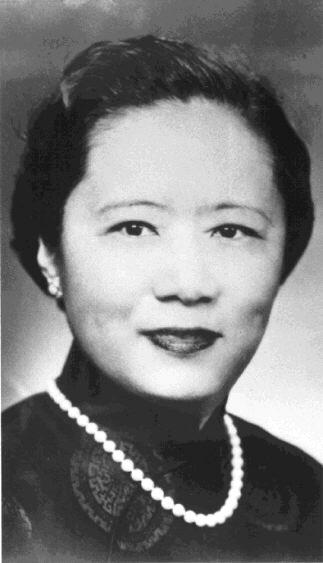
\includegraphics[width=0.3\textwidth]{fig/C_P_CP/Wu.jpg}
}&
\parbox{0.66\textwidth}{\textsf{\small
    ``Chien-Shiung Wu (often called "Madame Wu"), was born in Shanghai, China, in 1912. She
    received her Bachelor of Science degree in China in 1934 and came
    to the United States in 1936. After receiving her Ph.D. from the
    University of California in 1940, she taught at Smith College and
    at Princeton University before going to Columbia University in
    1944. As a nuclear physicist Dr. Wu worked on the Manhattan
    Project during the second World War. She became a professor of
    physics at Columbia and later held honorary professorships at
    several Chinese Universities. Dr. Wu received numerous honors and
    awards, including being the first woman elected president of the
    American Physical Society. She died in New York in February 1997.'' 
}}
\end{tabular}
\\  \textsf{Source: \httplink{http://www.physics.nist.gov/GenInt/Parity/people/Wu.html}}
\end{figure}
 Shortly after Young and Lee's proposal to search for parity violation in weak interactions, C.~S.~Wu, E.~Ambler, R.~W.~Hayward, D.~D.~Hoppes and
 R.~P.~Hudson showed in their
 \href{http://link.aps.org/abstract/PR/v105/p1413}{famous experiment}
 that parity is indeed
 violated\footnote{\href{http://link.aps.org/abstract/PR/v105/p1413}{C.S.~Wu, 
     E.~Ambler, R.W.~Hayward, D.D.~Hoppes and
     R.P.~Hudson Phys.~Rev.~{\bf 105},~1413~(157)}}.
\begin{figure}
\caption{Wu's Experiment}
\begin{tabular}{cc}
 Schematic & Not Wu \\
\parbox{0.49\textwidth}{
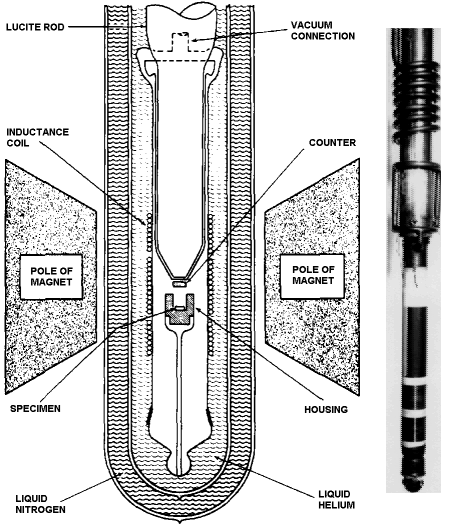
\includegraphics[width=0.49\textwidth]{fig/C_P_CP/wus_parity_apperatus.png}
}
&
\parbox{0.49\textwidth}{
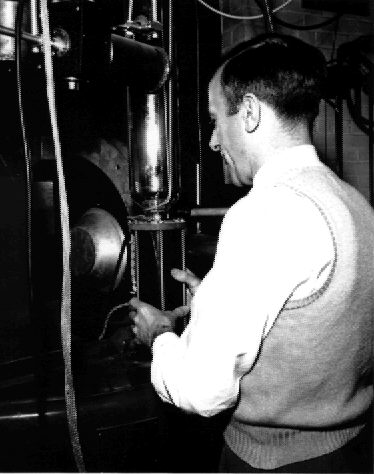
\includegraphics[width=0.49\textwidth]{fig/C_P_CP/wus_parity_photo.jpg}
}
\end{tabular}
\\Source:\href{http://physics.nist.gov/GenInt/Parity/expt.html#fig5-4-7}{\texttt{http://physics.nist.gov/GenInt/Parity/expt.html\#fig5-4-7}}
\end{figure}
 In the experiment, a sample of \chem{\mbox{}^{60}Co} is cooled down to
 very low temperatures, in a high magnetic field, and observed as it
 decays to \chem{\mbox{}^{60}Ni} under the emission of an electron and
 an (anti) neutrino. The observation was that the electrons were
 predominantly emitted opposite to the direction of the magnetic
 field. 
 %%
\begin{figure}
\centering
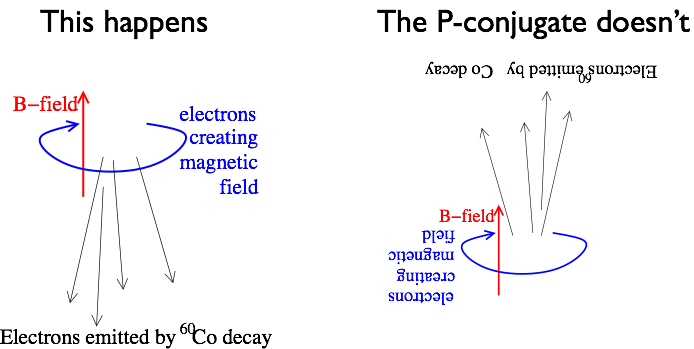
\includegraphics[width=0.8\textwidth]{fig/C_P_CP/0_MadamWuSchematic}
\caption{Schematic of Wu's experiment and how its P-conjugate would look like. Note that $\vec{B}$ does not change under \ps, while the momenta $\vec{p}$ do. So any momentum that is (always, or just preferentially) aligned with a $\vec{B}$ field must be \ps-violating. This is of course a simplified picture. In the real experiment, there would also be \emph{some} electrons that move in the other direction, along the $\vec{B}$ field (upwards in the picture on the left). This is because it is practically impossible to completely align the spins of the nuclei. But the observation of a significant up-down asymmetry in the electron direction is sufficient to prove \ps\ violation.
\label{fig:WuSchematic}}
\end{figure}
%%
\begin{figure}
\centering
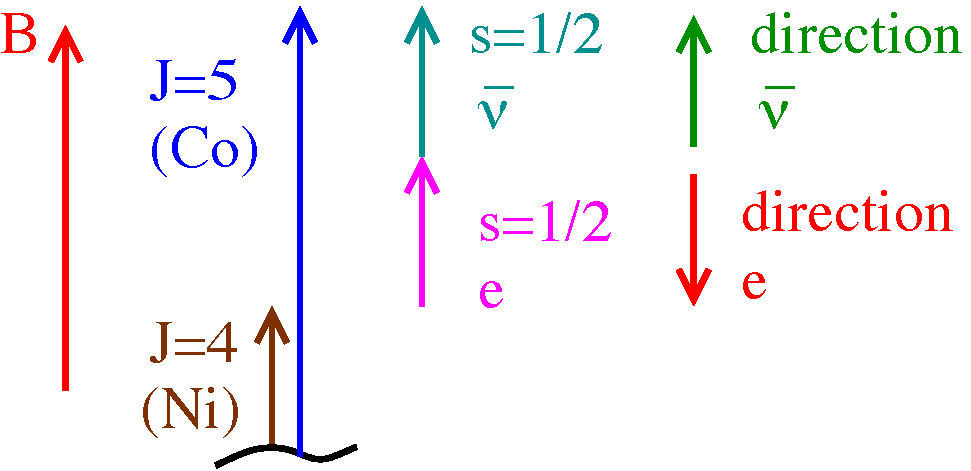
\includegraphics[width=0.8\textwidth]{fig/C_P_CP/0_MadamWuInterpretation}
\caption{Interpretation of Wu's experiment: The data can be explained if only (or at least preferentially) particles with negative helicity (spin opposite to the direction of motion, "left-handed particles") and anti-particles of positive helicity (right-handed particles) take part in the weak interaction. The true interpretation is not based on helicity, but the related, Lorentz-invariant quantity chirality.
\label{fig:WuInterpretation}}
\end{figure}
%%

